\documentclass[]{article}
\usepackage{lmodern}
\usepackage{amssymb,amsmath}
\usepackage{ifxetex,ifluatex}
\usepackage{fixltx2e} % provides \textsubscript
\ifnum 0\ifxetex 1\fi\ifluatex 1\fi=0 % if pdftex
  \usepackage[T1]{fontenc}
  \usepackage[utf8]{inputenc}
\else % if luatex or xelatex
  \ifxetex
    \usepackage{mathspec}
  \else
    \usepackage{fontspec}
  \fi
  \defaultfontfeatures{Ligatures=TeX,Scale=MatchLowercase}
\fi
% use upquote if available, for straight quotes in verbatim environments
\IfFileExists{upquote.sty}{\usepackage{upquote}}{}
% use microtype if available
\IfFileExists{microtype.sty}{%
\usepackage{microtype}
\UseMicrotypeSet[protrusion]{basicmath} % disable protrusion for tt fonts
}{}
\usepackage[margin=1in]{geometry}
\usepackage{hyperref}
\hypersetup{unicode=true,
            pdfborder={0 0 0},
            breaklinks=true}
\urlstyle{same}  % don't use monospace font for urls
\usepackage{color}
\usepackage{fancyvrb}
\newcommand{\VerbBar}{|}
\newcommand{\VERB}{\Verb[commandchars=\\\{\}]}
\DefineVerbatimEnvironment{Highlighting}{Verbatim}{commandchars=\\\{\}}
% Add ',fontsize=\small' for more characters per line
\usepackage{framed}
\definecolor{shadecolor}{RGB}{248,248,248}
\newenvironment{Shaded}{\begin{snugshade}}{\end{snugshade}}
\newcommand{\KeywordTok}[1]{\textcolor[rgb]{0.13,0.29,0.53}{\textbf{#1}}}
\newcommand{\DataTypeTok}[1]{\textcolor[rgb]{0.13,0.29,0.53}{#1}}
\newcommand{\DecValTok}[1]{\textcolor[rgb]{0.00,0.00,0.81}{#1}}
\newcommand{\BaseNTok}[1]{\textcolor[rgb]{0.00,0.00,0.81}{#1}}
\newcommand{\FloatTok}[1]{\textcolor[rgb]{0.00,0.00,0.81}{#1}}
\newcommand{\ConstantTok}[1]{\textcolor[rgb]{0.00,0.00,0.00}{#1}}
\newcommand{\CharTok}[1]{\textcolor[rgb]{0.31,0.60,0.02}{#1}}
\newcommand{\SpecialCharTok}[1]{\textcolor[rgb]{0.00,0.00,0.00}{#1}}
\newcommand{\StringTok}[1]{\textcolor[rgb]{0.31,0.60,0.02}{#1}}
\newcommand{\VerbatimStringTok}[1]{\textcolor[rgb]{0.31,0.60,0.02}{#1}}
\newcommand{\SpecialStringTok}[1]{\textcolor[rgb]{0.31,0.60,0.02}{#1}}
\newcommand{\ImportTok}[1]{#1}
\newcommand{\CommentTok}[1]{\textcolor[rgb]{0.56,0.35,0.01}{\textit{#1}}}
\newcommand{\DocumentationTok}[1]{\textcolor[rgb]{0.56,0.35,0.01}{\textbf{\textit{#1}}}}
\newcommand{\AnnotationTok}[1]{\textcolor[rgb]{0.56,0.35,0.01}{\textbf{\textit{#1}}}}
\newcommand{\CommentVarTok}[1]{\textcolor[rgb]{0.56,0.35,0.01}{\textbf{\textit{#1}}}}
\newcommand{\OtherTok}[1]{\textcolor[rgb]{0.56,0.35,0.01}{#1}}
\newcommand{\FunctionTok}[1]{\textcolor[rgb]{0.00,0.00,0.00}{#1}}
\newcommand{\VariableTok}[1]{\textcolor[rgb]{0.00,0.00,0.00}{#1}}
\newcommand{\ControlFlowTok}[1]{\textcolor[rgb]{0.13,0.29,0.53}{\textbf{#1}}}
\newcommand{\OperatorTok}[1]{\textcolor[rgb]{0.81,0.36,0.00}{\textbf{#1}}}
\newcommand{\BuiltInTok}[1]{#1}
\newcommand{\ExtensionTok}[1]{#1}
\newcommand{\PreprocessorTok}[1]{\textcolor[rgb]{0.56,0.35,0.01}{\textit{#1}}}
\newcommand{\AttributeTok}[1]{\textcolor[rgb]{0.77,0.63,0.00}{#1}}
\newcommand{\RegionMarkerTok}[1]{#1}
\newcommand{\InformationTok}[1]{\textcolor[rgb]{0.56,0.35,0.01}{\textbf{\textit{#1}}}}
\newcommand{\WarningTok}[1]{\textcolor[rgb]{0.56,0.35,0.01}{\textbf{\textit{#1}}}}
\newcommand{\AlertTok}[1]{\textcolor[rgb]{0.94,0.16,0.16}{#1}}
\newcommand{\ErrorTok}[1]{\textcolor[rgb]{0.64,0.00,0.00}{\textbf{#1}}}
\newcommand{\NormalTok}[1]{#1}
\usepackage{graphicx,grffile}
\makeatletter
\def\maxwidth{\ifdim\Gin@nat@width>\linewidth\linewidth\else\Gin@nat@width\fi}
\def\maxheight{\ifdim\Gin@nat@height>\textheight\textheight\else\Gin@nat@height\fi}
\makeatother
% Scale images if necessary, so that they will not overflow the page
% margins by default, and it is still possible to overwrite the defaults
% using explicit options in \includegraphics[width, height, ...]{}
\setkeys{Gin}{width=\maxwidth,height=\maxheight,keepaspectratio}
\IfFileExists{parskip.sty}{%
\usepackage{parskip}
}{% else
\setlength{\parindent}{0pt}
\setlength{\parskip}{6pt plus 2pt minus 1pt}
}
\setlength{\emergencystretch}{3em}  % prevent overfull lines
\providecommand{\tightlist}{%
  \setlength{\itemsep}{0pt}\setlength{\parskip}{0pt}}
\setcounter{secnumdepth}{0}
% Redefines (sub)paragraphs to behave more like sections
\ifx\paragraph\undefined\else
\let\oldparagraph\paragraph
\renewcommand{\paragraph}[1]{\oldparagraph{#1}\mbox{}}
\fi
\ifx\subparagraph\undefined\else
\let\oldsubparagraph\subparagraph
\renewcommand{\subparagraph}[1]{\oldsubparagraph{#1}\mbox{}}
\fi

%%% Use protect on footnotes to avoid problems with footnotes in titles
\let\rmarkdownfootnote\footnote%
\def\footnote{\protect\rmarkdownfootnote}

%%% Change title format to be more compact
\usepackage{titling}

% Create subtitle command for use in maketitle
\newcommand{\subtitle}[1]{
  \posttitle{
    \begin{center}\large#1\end{center}
    }
}

\setlength{\droptitle}{-2em}

  \title{}
    \pretitle{\vspace{\droptitle}}
  \posttitle{}
    \author{}
    \preauthor{}\postauthor{}
    \date{}
    \predate{}\postdate{}
  

\begin{document}

\begin{quote}
\emph{The power of intuitive understanding will protect you from harm until the end of your days.}
--- Lao Tzu
\end{quote}

\doublespacing

\section{Introduction}\label{introduction}

In 2012, Ford and Hill published an article that used some of the most
common approaches to mediation when a mediator and/or outcome is
categorical. Specifically, they used:

\begin{enumerate}
\def\labelenumi{\arabic{enumi}.}
\tightlist
\item
  the difference method {[}@mackinnon2008intro{]},
\item
  the ``categorical data method outlined by MacKinnon (2008)'' (pg. 5)
  to assess the significance of the difference method, and
\item
  the percent of the total effect that was mediated.
\end{enumerate}

These three approaches are not only common but likely some of the best
approaches in this situation. However, as stated in Chapter 4, these
have some notable shortcomings. First, the standard errors can be
inefficient and biased if there is a high degree of multi-collinearity
(or the degree to which there is perfect separability) in any of the
models.\footnote{Perfect separability is where a predictor can perfectly predict the outcome in logistic regression.}
The significance of the difference method depends on these standard
error estimates. Second, it does not provide the effect size measures
that would be most useful {[}e.g., the effect of increasing the
predictor on the outcome through the mediator(s){]}. Third, the
difference method is consistently too conservative with binary outcomes
{[}@Jiang2015{]}.

To build on the important findings from Ford and Hill (2012), this study
replicates their work using more recent data from 2014 while using MMA
to obtain effect sizes and confidence intervals for the indirect and
direct effects.

\section{Results}\label{results}

\begin{Shaded}
\begin{Highlighting}[]
\KeywordTok{library}\NormalTok{(tidyverse)}
\end{Highlighting}
\end{Shaded}

\begin{verbatim}
## Warning: package 'tidyverse' was built under R version 3.5.2
\end{verbatim}

\begin{verbatim}
## -- Attaching packages ------------------------------------------------------ tidyverse 1.2.1 --
\end{verbatim}

\begin{verbatim}
## v ggplot2 3.0.0     v purrr   0.2.5
## v tibble  1.4.2     v dplyr   0.7.6
## v tidyr   0.8.1     v stringr 1.3.1
## v readr   1.3.1     v forcats 0.3.0
\end{verbatim}

\begin{verbatim}
## Warning: package 'readr' was built under R version 3.5.2
\end{verbatim}

\begin{verbatim}
## Warning: package 'forcats' was built under R version 3.5.2
\end{verbatim}

\begin{verbatim}
## -- Conflicts --------------------------------------------------------- tidyverse_conflicts() --
## x dplyr::filter() masks stats::filter()
## x dplyr::lag()    masks stats::lag()
\end{verbatim}

\begin{Shaded}
\begin{Highlighting}[]
\KeywordTok{library}\NormalTok{(furniture)}
\end{Highlighting}
\end{Shaded}

\begin{verbatim}
## Warning: package 'furniture' was built under R version 3.5.2
\end{verbatim}

\begin{verbatim}
## -- furniture 1.8.7 ------------------------------------------ learn more at tysonbarrett.com --
## v furniture attached
## v No potential conflicts found
\end{verbatim}

\begin{Shaded}
\begin{Highlighting}[]
\NormalTok{## Load data}
\KeywordTok{load}\NormalTok{(}\StringTok{"Data/NSDUH_2014_Results.rda"}\NormalTok{)}
\NormalTok{d =}\StringTok{ }\NormalTok{da36361.}\DecValTok{0001}
\end{Highlighting}
\end{Shaded}

\begin{verbatim}
## Error in eval(expr, envir, enclos): object 'da36361.0001' not found
\end{verbatim}

\begin{Shaded}
\begin{Highlighting}[]
\KeywordTok{names}\NormalTok{(d) =}\StringTok{ }\KeywordTok{tolower}\NormalTok{(}\KeywordTok{names}\NormalTok{(d))}
\end{Highlighting}
\end{Shaded}

\begin{verbatim}
## Error in tolower(names(d)): object 'd' not found
\end{verbatim}

\begin{Shaded}
\begin{Highlighting}[]
\KeywordTok{rm}\NormalTok{(da36361.}\DecValTok{0001}\NormalTok{)}
\end{Highlighting}
\end{Shaded}

\begin{verbatim}
## Warning in rm(da36361.0001): object 'da36361.0001' not found
\end{verbatim}

\begin{Shaded}
\begin{Highlighting}[]
\NormalTok{## Variables}
\NormalTok{d1 =}\StringTok{ }\NormalTok{d }\OperatorTok
\StringTok{  }\KeywordTok{select}\NormalTok{(}
\NormalTok{    ## ----------------------------------- ##}
\NormalTok{    ##  Outcomes                           ##}
\NormalTok{    ##    (1,2,8,11,12 = within last year) ##}
\NormalTok{    ## ----------------------------------- ##}
\NormalTok{    ## Tobacco Outcome}
\NormalTok{    cigrec,    ## cig }
\NormalTok{    chewrec,   ## chew }
\NormalTok{    cigarrec,  ## cigar }
    \CommentTok{#pipe30dy,  ## pipe (30 days here instead)}
    
\NormalTok{    ## Heavy Drinking Outcome}
\NormalTok{    dr5day,  ## 1+ is within last 30 days}
    
\NormalTok{    ## Rx Outcome}
\NormalTok{    analrec, ## pain relievers}
\NormalTok{    tranrec, ## tranquilizers}
\NormalTok{    stimrec, ## stimulants}
\NormalTok{    sedrec,  ## sedatives}
    
\NormalTok{    ## Marijuana Outcome}
\NormalTok{    mjrec,   ## marijuana }
    
\NormalTok{    ## Other Illicit Outcome}
\NormalTok{    cocrec,  ## cocaine }
\NormalTok{    crakrec, ## crack }
\NormalTok{    herrec,  ## heroin }
\NormalTok{    hallrec, ## hallucinogens}
\NormalTok{    lsdrec,  ## LSD}
\NormalTok{    pcprec,  ## PCP}
\NormalTok{    ecsrec,  ## ecstacy}
\NormalTok{    inhrec,  ## inhalants}
\NormalTok{    methrec, ## meth}
    
\NormalTok{    ## ------------------------------------ ##}
\NormalTok{    ## Mediators                            ##}
\NormalTok{    ##   Mean response (higher = more cons) ##}
\NormalTok{    ## ------------------------------------ ##}
\NormalTok{    ## Self Views Mediator}
\NormalTok{    yegpkcig, ## someone your age cig}
\NormalTok{    yegmjevr, ## someone your age mj}
\NormalTok{    yegmjmo,  ## someone your age mj monthly}
\NormalTok{    yegaldly, ## someone your age drinking daily}
    
\NormalTok{    ## Peer Views Mediator}
\NormalTok{    yefpkcig, ## you cig}
\NormalTok{    yefmjevr, ## you mj}
\NormalTok{    yefmjmo,  ## you mj monthly}
\NormalTok{    yefaldly, ## you drinking daily}
    
\NormalTok{    ## Psychological Well-being (Major Depression)}
\NormalTok{    ymdeyr,  ## past year major depressive epidosde (MDE)}
    
\NormalTok{    ## ----------------------------------- ##}
\NormalTok{    ## Predictor                           ##}
\NormalTok{    ##   Cronbach's Alpha                  ##}
\NormalTok{    ##   Standardized mean level           ##}
\NormalTok{    ## ----------------------------------- ##}
\NormalTok{    ## Religiosity}
\NormalTok{    yerlgsvc, ## past 12, times at church (1-6}
\NormalTok{    yerlgimp, ## religious beliefs are important (1-4 strong dis to strong agree)}
\NormalTok{    yerldcsn, ## religious belief influence decisions (1-4)}
\NormalTok{    yefaiact, ## religious activities}
    
\NormalTok{    ## ----------------------------------- ##}
\NormalTok{    ## Control Variables                   ##}
\NormalTok{    ## ----------------------------------- ##}
\NormalTok{    ## Parental Attitudes}
\NormalTok{    yeppkcig, ## parents feel about cig}
\NormalTok{    yepmjevr, ## parents feel about mj}
\NormalTok{    yepmjmo,  ## parents feel about mj monthly}
\NormalTok{    yepaldly, ## parents feel about drinking daily}
    
\NormalTok{    ## Demographics}
\NormalTok{    age2,    ## age}
\NormalTok{    catage,  ## age category (1 = 12-17 year old)}
\NormalTok{    irsex,   ## gender (1 = male)}
\NormalTok{    newrace2, ## race (1 = White, 2-7 non-white)}
\NormalTok{    irfamin3, ## total family income (6 = 50,000 - 74,999)}
\NormalTok{    poverty2, ## not used in the study but could be for ours }
\NormalTok{              ##  (1 = poverty, 2 = low middle, 3 = middle class or more)}
    
\NormalTok{    ## ----------------------------------- ##}
\NormalTok{    ## Sampling Variables                  ##}
\NormalTok{    ## ----------------------------------- ##}
\NormalTok{    analwt_c,  ## sample weight}
\NormalTok{    vestr,     ## analysis stratum}
\NormalTok{    verep      ## analysis replicate}
\NormalTok{    ) }\OperatorTok
\StringTok{  }\KeywordTok{filter}\NormalTok{(catage }\OperatorTok{==}\StringTok{ "(1) 12-17 Years Old"}\NormalTok{)}
\end{Highlighting}
\end{Shaded}

\begin{verbatim}
## Error in eval(lhs, parent, parent): object 'd' not found
\end{verbatim}

\begin{Shaded}
\begin{Highlighting}[]
\NormalTok{## Data Cleaning}
\NormalTok{dich =}\StringTok{ }\ControlFlowTok{function}\NormalTok{(x)\{}
\NormalTok{  x =}\StringTok{ }\KeywordTok{ifelse}\NormalTok{(}\KeywordTok{grepl}\NormalTok{(}\StringTok{"(01)|(02)|(08)|(11)"}\NormalTok{, x), }\DecValTok{1}\NormalTok{, }\DecValTok{0}\NormalTok{)}
\NormalTok{  x}
\NormalTok{\}}
\NormalTok{map_to =}\StringTok{ }\ControlFlowTok{function}\NormalTok{(x)\{}
\NormalTok{  lbls =}\StringTok{ }\KeywordTok{sort}\NormalTok{(}\KeywordTok{levels}\NormalTok{(x))}
\NormalTok{  lbls =}\StringTok{ }\NormalTok{(}\KeywordTok{sub}\NormalTok{(}\StringTok{"^}\CharTok{\textbackslash{}\textbackslash{}}\StringTok{([0-9]+}\CharTok{\textbackslash{}\textbackslash{}}\StringTok{) +(.+$)"}\NormalTok{, }\StringTok{"}\CharTok{\textbackslash{}\textbackslash{}}\StringTok{1"}\NormalTok{, lbls))}
\NormalTok{  x =}\StringTok{ }\KeywordTok{as.numeric}\NormalTok{(}\KeywordTok{gsub}\NormalTok{(}\StringTok{"^}\CharTok{\textbackslash{}\textbackslash{}}\StringTok{(0*([0-9]+)}\CharTok{\textbackslash{}\textbackslash{}}\StringTok{).+$"}\NormalTok{, }\StringTok{"}\CharTok{\textbackslash{}\textbackslash{}}\StringTok{1"}\NormalTok{, x))}
\NormalTok{  x}
\NormalTok{\}}
\NormalTok{d1[, }\KeywordTok{c}\NormalTok{(}\DecValTok{1}\OperatorTok{:}\DecValTok{18}\NormalTok{)]  =}\StringTok{ }\KeywordTok{map_df}\NormalTok{(d1[, }\KeywordTok{c}\NormalTok{(}\DecValTok{1}\OperatorTok{:}\DecValTok{18}\NormalTok{)], }\OperatorTok{~}\KeywordTok{dich}\NormalTok{(.x))}
\end{Highlighting}
\end{Shaded}

\begin{verbatim}
## Error in map(.x, .f, ...): object 'd1' not found
\end{verbatim}

\begin{Shaded}
\begin{Highlighting}[]
\NormalTok{d1[, }\KeywordTok{c}\NormalTok{(}\DecValTok{19}\OperatorTok{:}\DecValTok{36}\NormalTok{)] =}\StringTok{ }\KeywordTok{map_if}\NormalTok{(d1[, }\KeywordTok{c}\NormalTok{(}\DecValTok{19}\OperatorTok{:}\DecValTok{36}\NormalTok{)], is.factor, }\OperatorTok{~}\KeywordTok{map_to}\NormalTok{(.x))}
\end{Highlighting}
\end{Shaded}

\begin{verbatim}
## Error in map_lgl(.x, .p, ...): object 'd1' not found
\end{verbatim}

\begin{Shaded}
\begin{Highlighting}[]
\NormalTok{## Creating final modeling variables}
\NormalTok{d1 =}\StringTok{ }\NormalTok{d1 }\OperatorTok
\StringTok{  }\KeywordTok{mutate}\NormalTok{(}\DataTypeTok{tobacco =} \KeywordTok{ifelse}\NormalTok{(}\KeywordTok{rowSums}\NormalTok{(}\KeywordTok{cbind}\NormalTok{(cigrec, chewrec, }
\NormalTok{                                        cigarrec)) }\OperatorTok{>}\StringTok{ }\DecValTok{0}\NormalTok{, }\DecValTok{1}\NormalTok{, }\DecValTok{0}\NormalTok{),}
         \DataTypeTok{drink   =}\NormalTok{ dr5day,}
         \DataTypeTok{rx      =} \KeywordTok{ifelse}\NormalTok{(}\KeywordTok{rowSums}\NormalTok{(}\KeywordTok{cbind}\NormalTok{(analrec, tranrec, }
\NormalTok{                                        stimrec, sedrec)) }\OperatorTok{>}\StringTok{ }\DecValTok{0}\NormalTok{, }\DecValTok{1}\NormalTok{, }\DecValTok{0}\NormalTok{),}
         \DataTypeTok{mari    =} \KeywordTok{ifelse}\NormalTok{(mjrec }\OperatorTok{==}\StringTok{ }\DecValTok{1}\NormalTok{, }\DecValTok{1}\NormalTok{, }\DecValTok{0}\NormalTok{),}
         \DataTypeTok{illicit =} \KeywordTok{ifelse}\NormalTok{(}\KeywordTok{rowSums}\NormalTok{(}\KeywordTok{cbind}\NormalTok{(cocrec, crakrec, }
\NormalTok{                                        herrec, hallrec,}
\NormalTok{                                        lsdrec, pcprec, }
\NormalTok{                                        ecsrec, inhrec, }
\NormalTok{                                        methrec)) }\OperatorTok{>}\StringTok{ }\DecValTok{0}\NormalTok{, }\DecValTok{1}\NormalTok{, }\DecValTok{0}\NormalTok{)) }\OperatorTok
\StringTok{  }\KeywordTok{mutate}\NormalTok{(}\DataTypeTok{self =} \KeywordTok{rowMeans}\NormalTok{(}\KeywordTok{cbind}\NormalTok{(yegpkcig, yegmjevr, yegmjmo, yegaldly)),}
         \DataTypeTok{peer =} \KeywordTok{rowMeans}\NormalTok{(}\KeywordTok{cbind}\NormalTok{(yefpkcig, yefmjevr, yefmjmo, yefaldly))) }\OperatorTok
\StringTok{  }\KeywordTok{mutate}\NormalTok{(}\DataTypeTok{dep =} \KeywordTok{washer}\NormalTok{(ymdeyr, }\DecValTok{2}\NormalTok{, }\DataTypeTok{value =} \DecValTok{0}\NormalTok{)) }\OperatorTok
\StringTok{  }\KeywordTok{mutate}\NormalTok{(}\DataTypeTok{religious =} \KeywordTok{rowMeans}\NormalTok{(}\KeywordTok{cbind}\NormalTok{(}\KeywordTok{scale}\NormalTok{(yerlgsvc),}
                                    \KeywordTok{scale}\NormalTok{(yerlgimp),}
                                    \KeywordTok{scale}\NormalTok{(yerldcsn), }
                                    \KeywordTok{scale}\NormalTok{(yefaiact)))) }\OperatorTok
\StringTok{  }\KeywordTok{mutate}\NormalTok{(}\DataTypeTok{parent =} \KeywordTok{rowMeans}\NormalTok{(}\KeywordTok{cbind}\NormalTok{(yeppkcig, yepmjevr, }
\NormalTok{                                 yepmjmo, yepaldly)))}
\end{Highlighting}
\end{Shaded}

\begin{verbatim}
## Error in eval(lhs, parent, parent): object 'd1' not found
\end{verbatim}

\begin{Shaded}
\begin{Highlighting}[]
\NormalTok{## Sampling Design}
\KeywordTok{library}\NormalTok{(survey)}
\NormalTok{design =}\StringTok{ }\KeywordTok{svydesign}\NormalTok{(}\DataTypeTok{ids =} \OperatorTok{~}\DecValTok{1}\NormalTok{, }
                   \DataTypeTok{strata =} \OperatorTok{~}\NormalTok{vestr, }
                   \DataTypeTok{weights =} \OperatorTok{~}\NormalTok{analwt_c,}
                   \DataTypeTok{data =}\NormalTok{ d1)}

\NormalTok{## All a Path Models}
\NormalTok{## Unadjusted}
\NormalTok{svy_a1 =}\StringTok{ }\KeywordTok{svyglm}\NormalTok{(self }\OperatorTok{~}\StringTok{ }\NormalTok{religious, }\DataTypeTok{design =}\NormalTok{ design)}
\NormalTok{svy_a2 =}\StringTok{ }\KeywordTok{svyglm}\NormalTok{(peer }\OperatorTok{~}\StringTok{ }\NormalTok{religious, }\DataTypeTok{design =}\NormalTok{ design)}
\NormalTok{svy_a3 =}\StringTok{ }\KeywordTok{svyglm}\NormalTok{(dep }\OperatorTok{~}\StringTok{ }\NormalTok{religious, }\DataTypeTok{design =}\NormalTok{ design, }
                \DataTypeTok{family =} \StringTok{'quasibinomial'}\NormalTok{)}

\NormalTok{## Adjusted}
\NormalTok{svy_a12 =}\StringTok{ }\KeywordTok{svyglm}\NormalTok{(self }\OperatorTok{~}\StringTok{ }\NormalTok{religious }\OperatorTok{+}\StringTok{ }\NormalTok{age2 }\OperatorTok{+}\StringTok{ }
\StringTok{                   }\NormalTok{irsex }\OperatorTok{+}\StringTok{ }\NormalTok{newrace2 }\OperatorTok{+}\StringTok{ }\NormalTok{irfamin3 }\OperatorTok{+}\StringTok{ }\NormalTok{parent, }
                 \DataTypeTok{design =}\NormalTok{ design)}
\NormalTok{svy_a22 =}\StringTok{ }\KeywordTok{svyglm}\NormalTok{(peer }\OperatorTok{~}\StringTok{ }\NormalTok{religious }\OperatorTok{+}\StringTok{ }\NormalTok{age2 }\OperatorTok{+}\StringTok{ }
\StringTok{                   }\NormalTok{irsex }\OperatorTok{+}\StringTok{ }\NormalTok{newrace2 }\OperatorTok{+}\StringTok{ }\NormalTok{irfamin3 }\OperatorTok{+}\StringTok{ }\NormalTok{parent, }
                 \DataTypeTok{design =}\NormalTok{ design)}
\NormalTok{svy_a32 =}\StringTok{ }\KeywordTok{svyglm}\NormalTok{(dep }\OperatorTok{~}\StringTok{ }\NormalTok{religious }\OperatorTok{+}\StringTok{ }\NormalTok{age2 }\OperatorTok{+}\StringTok{ }
\StringTok{                   }\NormalTok{irsex }\OperatorTok{+}\StringTok{ }\NormalTok{newrace2 }\OperatorTok{+}\StringTok{ }\NormalTok{irfamin3 }\OperatorTok{+}\StringTok{ }\NormalTok{parent, }
                 \DataTypeTok{design =}\NormalTok{ design, }
                 \DataTypeTok{family =} \StringTok{'quasibinomial'}\NormalTok{)}

\NormalTok{## All b and c' Path Models (drink such low prevalence that it was not included)}
\NormalTok{svy_bc =}\StringTok{ }\NormalTok{svy_bc2 =}\StringTok{ }\KeywordTok{list}\NormalTok{()}
\ControlFlowTok{for}\NormalTok{ (i }\ControlFlowTok{in} \KeywordTok{c}\NormalTok{(}\StringTok{"tobacco"}\NormalTok{, }\StringTok{"rx"}\NormalTok{, }\StringTok{"mari"}\NormalTok{, }\StringTok{"illicit"}\NormalTok{))\{}
  
\NormalTok{  ## Unadjusted Model}
\NormalTok{  model =}\StringTok{ }\KeywordTok{as.formula}\NormalTok{(}\KeywordTok{paste0}\NormalTok{(i, }\StringTok{"~ self + peer + dep + religious"}\NormalTok{))}
\NormalTok{  svy_bc[[i]] =}\StringTok{ }\KeywordTok{svyglm}\NormalTok{(model, }\DataTypeTok{design =}\NormalTok{ design, }\DataTypeTok{family =} \StringTok{"binomial"}\NormalTok{)}
  
\NormalTok{  ## Adjusted Model}
\NormalTok{  model2 =}\StringTok{ }\KeywordTok{as.formula}\NormalTok{(}\KeywordTok{paste0}\NormalTok{(i, }\StringTok{"~ self + peer + dep + religious + age2 + }
\StringTok{                             irsex + newrace2 + irfamin3 + parent"}\NormalTok{))}
\NormalTok{  svy_bc2[[i]] =}\StringTok{ }\KeywordTok{svyglm}\NormalTok{(model2, }\DataTypeTok{design =}\NormalTok{ design, }\DataTypeTok{family =} \StringTok{"binomial"}\NormalTok{)}
  
\NormalTok{\}}

\KeywordTok{library}\NormalTok{(MarginalMediation)}
\NormalTok{## Tobacco}
\NormalTok{fit_tob =}\StringTok{ }\KeywordTok{mma}\NormalTok{(svy_bc[[}\StringTok{"tobacco"}\NormalTok{]],}
\NormalTok{              svy_a1,}
\NormalTok{              svy_a2,}
\NormalTok{              svy_a3,}
              \DataTypeTok{ind_effects =} \KeywordTok{c}\NormalTok{(}\StringTok{"religious-self"}\NormalTok{,}
                              \StringTok{"religious-peer"}\NormalTok{,}
                              \StringTok{"religious-dep"}\NormalTok{),}
              \DataTypeTok{boot =} \DecValTok{500}\NormalTok{)}
\NormalTok{fit_tob2 =}\StringTok{ }\KeywordTok{mma}\NormalTok{(svy_bc2[[}\StringTok{"tobacco"}\NormalTok{]],}
\NormalTok{               svy_a12,}
\NormalTok{               svy_a22,}
\NormalTok{               svy_a32,}
               \DataTypeTok{ind_effects =} \KeywordTok{c}\NormalTok{(}\StringTok{"religious-self"}\NormalTok{,}
                               \StringTok{"religious-peer"}\NormalTok{,}
                               \StringTok{"religious-dep"}\NormalTok{),}
               \DataTypeTok{boot =} \DecValTok{500}\NormalTok{)}

\NormalTok{## Rx}
\NormalTok{fit_rx =}\StringTok{ }\KeywordTok{mma}\NormalTok{(svy_bc[[}\StringTok{"rx"}\NormalTok{]],}
\NormalTok{              svy_a1,}
\NormalTok{              svy_a2,}
\NormalTok{              svy_a3,}
              \DataTypeTok{ind_effects =} \KeywordTok{c}\NormalTok{(}\StringTok{"religious-self"}\NormalTok{,}
                              \StringTok{"religious-peer"}\NormalTok{,}
                              \StringTok{"religious-dep"}\NormalTok{),}
              \DataTypeTok{boot =} \DecValTok{500}\NormalTok{)}
\NormalTok{fit_rx2 =}\StringTok{ }\KeywordTok{mma}\NormalTok{(svy_bc2[[}\StringTok{"rx"}\NormalTok{]],}
\NormalTok{               svy_a12,}
\NormalTok{               svy_a22,}
\NormalTok{               svy_a32,}
               \DataTypeTok{ind_effects =} \KeywordTok{c}\NormalTok{(}\StringTok{"religious-self"}\NormalTok{,}
                               \StringTok{"religious-peer"}\NormalTok{,}
                               \StringTok{"religious-dep"}\NormalTok{),}
               \DataTypeTok{boot =} \DecValTok{500}\NormalTok{)}

\NormalTok{## Marijuana}
\NormalTok{fit_mar =}\StringTok{ }\KeywordTok{mma}\NormalTok{(svy_bc[[}\StringTok{"mari"}\NormalTok{]],}
\NormalTok{             svy_a1,}
\NormalTok{             svy_a2,}
\NormalTok{             svy_a3,}
             \DataTypeTok{ind_effects =} \KeywordTok{c}\NormalTok{(}\StringTok{"religious-self"}\NormalTok{,}
                             \StringTok{"religious-peer"}\NormalTok{,}
                             \StringTok{"religious-dep"}\NormalTok{),}
             \DataTypeTok{boot =} \DecValTok{500}\NormalTok{)}
\NormalTok{fit_mar2 =}\StringTok{ }\KeywordTok{mma}\NormalTok{(svy_bc2[[}\StringTok{"mari"}\NormalTok{]],}
\NormalTok{              svy_a12,}
\NormalTok{              svy_a22,}
\NormalTok{              svy_a32,}
              \DataTypeTok{ind_effects =} \KeywordTok{c}\NormalTok{(}\StringTok{"religious-self"}\NormalTok{,}
                              \StringTok{"religious-peer"}\NormalTok{,}
                              \StringTok{"religious-dep"}\NormalTok{),}
              \DataTypeTok{boot =} \DecValTok{500}\NormalTok{)}

\NormalTok{## Illicit}
\NormalTok{fit_ill =}\StringTok{ }\KeywordTok{mma}\NormalTok{(svy_bc[[}\StringTok{"illicit"}\NormalTok{]],}
\NormalTok{              svy_a1,}
\NormalTok{              svy_a2,}
\NormalTok{              svy_a3,}
              \DataTypeTok{ind_effects =} \KeywordTok{c}\NormalTok{(}\StringTok{"religious-self"}\NormalTok{,}
                              \StringTok{"religious-peer"}\NormalTok{,}
                              \StringTok{"religious-dep"}\NormalTok{),}
              \DataTypeTok{boot =} \DecValTok{500}\NormalTok{)}
\NormalTok{fit_ill2 =}\StringTok{ }\KeywordTok{mma}\NormalTok{(svy_bc2[[}\StringTok{"illicit"}\NormalTok{]],}
\NormalTok{               svy_a12,}
\NormalTok{               svy_a22,}
\NormalTok{               svy_a32,}
               \DataTypeTok{ind_effects =} \KeywordTok{c}\NormalTok{(}\StringTok{"religious-self"}\NormalTok{,}
                               \StringTok{"religious-peer"}\NormalTok{,}
                               \StringTok{"religious-dep"}\NormalTok{),}
               \DataTypeTok{boot =} \DecValTok{500}\NormalTok{)}

\KeywordTok{save}\NormalTok{(fit_tob, fit_tob2, }
\NormalTok{     fit_rx, fit_rx2, }
\NormalTok{     fit_mar, fit_mar2, }
\NormalTok{     fit_ill, fit_ill2,}
     \DataTypeTok{file =} \KeywordTok{here}\NormalTok{(}\StringTok{"Data/NSDUH_2014_Results.rda"}\NormalTok{))}
\end{Highlighting}
\end{Shaded}

\begin{Shaded}
\begin{Highlighting}[]
\KeywordTok{library}\NormalTok{(MarginalMediation)}
\end{Highlighting}
\end{Shaded}

\begin{verbatim}
## Warning: package 'MarginalMediation' was built under R version 3.5.2
\end{verbatim}

\begin{verbatim}
## MarginalMediation 0.5.1: Please report any bugs (t.barrett@aggiemail.usu.edu).
\end{verbatim}

\begin{Shaded}
\begin{Highlighting}[]
\KeywordTok{library}\NormalTok{(tidyverse)}
\KeywordTok{library}\NormalTok{(here)}
\end{Highlighting}
\end{Shaded}

\begin{verbatim}
## Error in library(here): there is no package called 'here'
\end{verbatim}

\begin{Shaded}
\begin{Highlighting}[]
\KeywordTok{load}\NormalTok{(}\DataTypeTok{file =} \KeywordTok{here}\NormalTok{(}\StringTok{"Data/NSDUH_2014_Results.rda"}\NormalTok{))}
\end{Highlighting}
\end{Shaded}

\begin{verbatim}
## Error in here("Data/NSDUH_2014_Results.rda"): could not find function "here"
\end{verbatim}

\begin{Shaded}
\begin{Highlighting}[]
\NormalTok{## Extract direct effects}
\NormalTok{directs_fx =}\StringTok{ }\ControlFlowTok{function}\NormalTok{(..., type)\{}
  \KeywordTok{list}\NormalTok{(...) }\OperatorTok
\StringTok{    }\KeywordTok{map}\NormalTok{(}\OperatorTok{~}\NormalTok{.x}\OperatorTok{$}\NormalTok{dir_effects) }\OperatorTok
\StringTok{    }\KeywordTok{do.call}\NormalTok{(}\StringTok{"rbind"}\NormalTok{, .) }\OperatorTok
\StringTok{    }\KeywordTok{data.frame}\NormalTok{(.) }\OperatorTok
\StringTok{    }\KeywordTok{select}\NormalTok{(Direct, Lower, Upper) }\OperatorTok
\StringTok{    }\KeywordTok{data.frame}\NormalTok{(., }\DataTypeTok{row.names =} 
                 \KeywordTok{gsub}\NormalTok{(}\StringTok{"religious"}\NormalTok{, }\StringTok{"Religiousity (Direct)"}\NormalTok{, }\KeywordTok{row.names}\NormalTok{(.))) }\OperatorTok
\StringTok{    }\KeywordTok{rownames_to_column}\NormalTok{() }\OperatorTok
\StringTok{    }\KeywordTok{mutate}\NormalTok{(}\DataTypeTok{Outcome =} \KeywordTok{c}\NormalTok{(}\KeywordTok{rep}\NormalTok{(}\StringTok{"Tobacco"}\NormalTok{, }\DecValTok{1}\NormalTok{), }\KeywordTok{rep}\NormalTok{(}\StringTok{"Prescription"}\NormalTok{, }\DecValTok{1}\NormalTok{),}
                       \KeywordTok{rep}\NormalTok{(}\StringTok{"Marijuana"}\NormalTok{, }\DecValTok{1}\NormalTok{), }\KeywordTok{rep}\NormalTok{(}\StringTok{"Illicit"}\NormalTok{, }\DecValTok{1}\NormalTok{))) }\OperatorTok\StringTok{  }
\StringTok{    }\KeywordTok{select}\NormalTok{(Outcome, rowname, Direct, Lower, Upper) }\OperatorTok
\StringTok{    }\KeywordTok{set_names}\NormalTok{(}\KeywordTok{c}\NormalTok{(}\StringTok{"Outcome"}\NormalTok{, }\StringTok{"Path"}\NormalTok{, }\StringTok{"Estimate"}\NormalTok{, }\StringTok{"Lower"}\NormalTok{, }\StringTok{"Upper"}\NormalTok{)) }\OperatorTok
\StringTok{    }\KeywordTok{mutate}\NormalTok{(}\DataTypeTok{CI =} \KeywordTok{paste0}\NormalTok{(}\StringTok{"("}\NormalTok{, }\KeywordTok{round}\NormalTok{(Lower,}\DecValTok{4}\NormalTok{), }\StringTok{", "}\NormalTok{, }\KeywordTok{round}\NormalTok{(Upper,}\DecValTok{4}\NormalTok{), }\StringTok{")"}\NormalTok{)) }\OperatorTok
\StringTok{    }\KeywordTok{select}\NormalTok{(}\OperatorTok{-}\NormalTok{CI) }\OperatorTok
\StringTok{    }\KeywordTok{mutate}\NormalTok{(}\DataTypeTok{type =}\NormalTok{ type)}
\NormalTok{\}}
\NormalTok{directs_un =}\StringTok{ }\KeywordTok{directs_fx}\NormalTok{(fit_tob, }
\NormalTok{                        fit_rx, }
\NormalTok{                        fit_mar, }
\NormalTok{                        fit_ill, }
                        \DataTypeTok{type =} \StringTok{"Unadjusted"}\NormalTok{)}
\NormalTok{directs_adj =}\StringTok{ }\KeywordTok{directs_fx}\NormalTok{(fit_tob2, }
\NormalTok{                         fit_rx2, }
\NormalTok{                         fit_mar2, }
\NormalTok{                         fit_ill2, }
                         \DataTypeTok{type =} \StringTok{"Adjusted"}\NormalTok{)}

\NormalTok{## Extract indirect effects and bind to directs}
\NormalTok{inds_fx =}\StringTok{ }\ControlFlowTok{function}\NormalTok{(..., type)\{}
  \KeywordTok{list}\NormalTok{(...) }\OperatorTok
\StringTok{    }\KeywordTok{map}\NormalTok{(}\OperatorTok{~}\NormalTok{.x}\OperatorTok{$}\NormalTok{ind_effects) }\OperatorTok
\StringTok{    }\KeywordTok{do.call}\NormalTok{(}\StringTok{"rbind"}\NormalTok{, .) }\OperatorTok
\StringTok{    }\KeywordTok{data.frame}\NormalTok{(.) }\OperatorTok
\StringTok{    }\KeywordTok{select}\NormalTok{(Indirect, Lower, Upper) }\OperatorTok
\StringTok{    }\KeywordTok{data.frame}\NormalTok{(., }\DataTypeTok{row.names =} \KeywordTok{gsub}\NormalTok{(}\StringTok{"religious-"}\NormalTok{, }\StringTok{"Religiousity Through"}\NormalTok{, }
                                   \KeywordTok{row.names}\NormalTok{(.))) }\OperatorTok
\StringTok{    }\KeywordTok{data.frame}\NormalTok{(., }\DataTypeTok{row.names =} \KeywordTok{gsub}\NormalTok{(}\StringTok{"dep"}\NormalTok{, }\StringTok{"}\CharTok{\textbackslash{}n}\StringTok{Depression"}\NormalTok{, }
                                   \KeywordTok{row.names}\NormalTok{(.))) }\OperatorTok
\StringTok{    }\KeywordTok{data.frame}\NormalTok{(., }\DataTypeTok{row.names =} \KeywordTok{gsub}\NormalTok{(}\StringTok{"self"}\NormalTok{, }\StringTok{"}\CharTok{\textbackslash{}n}\StringTok{Respondent Views"}\NormalTok{, }
                                   \KeywordTok{row.names}\NormalTok{(.))) }\OperatorTok
\StringTok{    }\KeywordTok{data.frame}\NormalTok{(., }\DataTypeTok{row.names =} \KeywordTok{gsub}\NormalTok{(}\StringTok{"peer"}\NormalTok{, }\StringTok{"}\CharTok{\textbackslash{}n}\StringTok{Peer Views"}\NormalTok{, }
                                   \KeywordTok{row.names}\NormalTok{(.))) }\OperatorTok
\StringTok{    }\KeywordTok{rownames_to_column}\NormalTok{() }\OperatorTok
\StringTok{    }\KeywordTok{mutate}\NormalTok{(}\DataTypeTok{Outcome =} \KeywordTok{c}\NormalTok{(}\KeywordTok{rep}\NormalTok{(}\StringTok{"Tobacco"}\NormalTok{, }\DecValTok{3}\NormalTok{), }
                       \KeywordTok{rep}\NormalTok{(}\StringTok{"Prescription"}\NormalTok{, }\DecValTok{3}\NormalTok{),}
                       \KeywordTok{rep}\NormalTok{(}\StringTok{"Marijuana"}\NormalTok{, }\DecValTok{3}\NormalTok{), }
                       \KeywordTok{rep}\NormalTok{(}\StringTok{"Illicit"}\NormalTok{, }\DecValTok{3}\NormalTok{))) }\OperatorTok
\StringTok{    }\KeywordTok{select}\NormalTok{(Outcome, rowname, Indirect, Lower, Upper) }\OperatorTok
\StringTok{    }\KeywordTok{set_names}\NormalTok{(}\KeywordTok{c}\NormalTok{(}\StringTok{"Outcome"}\NormalTok{, }\StringTok{"Path"}\NormalTok{, }\StringTok{"Estimate"}\NormalTok{, }
                \StringTok{"Lower"}\NormalTok{, }\StringTok{"Upper"}\NormalTok{)) }\OperatorTok
\StringTok{    }\KeywordTok{mutate}\NormalTok{(}\DataTypeTok{CI =} \KeywordTok{paste0}\NormalTok{(}\StringTok{"("}\NormalTok{, }\KeywordTok{round}\NormalTok{(Lower,}\DecValTok{4}\NormalTok{), }\StringTok{", "}\NormalTok{, }
                       \KeywordTok{round}\NormalTok{(Upper,}\DecValTok{4}\NormalTok{), }\StringTok{")"}\NormalTok{)) }\OperatorTok
\StringTok{    }\KeywordTok{select}\NormalTok{(}\OperatorTok{-}\NormalTok{CI) }\OperatorTok
\StringTok{    }\KeywordTok{mutate}\NormalTok{(}\DataTypeTok{type =}\NormalTok{ type)}
\NormalTok{\}}
\NormalTok{unadjusted =}\StringTok{ }\KeywordTok{inds_fx}\NormalTok{(fit_tob, }
\NormalTok{                     fit_rx, }
\NormalTok{                     fit_mar, }
\NormalTok{                     fit_ill, }
                     \DataTypeTok{type =} \StringTok{"Unadjusted"}\NormalTok{) }\OperatorTok
\StringTok{  }\KeywordTok{rbind}\NormalTok{(directs_un)}
\NormalTok{adjusted =}\StringTok{ }\KeywordTok{inds_fx}\NormalTok{(fit_tob2, }
\NormalTok{                   fit_rx2, }
\NormalTok{                   fit_mar2, }
\NormalTok{                   fit_ill2, }
                   \DataTypeTok{type =} \StringTok{"Adjusted"}\NormalTok{) }\OperatorTok
\StringTok{  }\KeywordTok{rbind}\NormalTok{(directs_adj)}
\NormalTok{inds =}\StringTok{ }\KeywordTok{rbind}\NormalTok{(unadjusted, adjusted) }\OperatorTok
\StringTok{  }\NormalTok{data.frame }\OperatorTok
\StringTok{  }\KeywordTok{mutate}\NormalTok{(}\DataTypeTok{type =} \KeywordTok{factor}\NormalTok{(type, }
                       \DataTypeTok{levels =} \KeywordTok{c}\NormalTok{(}\StringTok{"Unadjusted"}\NormalTok{, }\StringTok{"Adjusted"}\NormalTok{))) }\OperatorTok
\StringTok{  }\KeywordTok{mutate}\NormalTok{(}\DataTypeTok{Path =} \KeywordTok{gsub}\NormalTok{(}\StringTok{"[0-9]"}\NormalTok{,}\StringTok{""}\NormalTok{, Path)) }\OperatorTok
\StringTok{  }\KeywordTok{mutate}\NormalTok{(}\DataTypeTok{Outcome =} \KeywordTok{factor}\NormalTok{(Outcome, }
                          \DataTypeTok{levels =} \KeywordTok{c}\NormalTok{(}\StringTok{"Tobacco"}\NormalTok{, }\StringTok{"Prescription"}\NormalTok{,}
                                     \StringTok{"Marijuana"}\NormalTok{, }\StringTok{"Illicit"}\NormalTok{)))}
\end{Highlighting}
\end{Shaded}

\begin{Shaded}
\begin{Highlighting}[]
\NormalTok{## Odds ratios and linear effects as done in Ford and Hill}
\NormalTok{## Sampling Design}
\KeywordTok{library}\NormalTok{(survey)}
\end{Highlighting}
\end{Shaded}

\begin{verbatim}
## Error in library(survey): there is no package called 'survey'
\end{verbatim}

\begin{Shaded}
\begin{Highlighting}[]
\NormalTok{design =}\StringTok{ }\KeywordTok{svydesign}\NormalTok{(}\DataTypeTok{ids =} \OperatorTok{~}\DecValTok{1}\NormalTok{, }
                   \DataTypeTok{strata =} \OperatorTok{~}\NormalTok{vestr, }
                   \DataTypeTok{weights =} \OperatorTok{~}\NormalTok{analwt_c,}
                   \DataTypeTok{data =}\NormalTok{ d1)}
\end{Highlighting}
\end{Shaded}

\begin{verbatim}
## Error in svydesign(ids = ~1, strata = ~vestr, weights = ~analwt_c, data = d1): could not find function "svydesign"
\end{verbatim}

\begin{Shaded}
\begin{Highlighting}[]
\NormalTok{## All a Path Models}
\NormalTok{svy_a1 =}\StringTok{ }\KeywordTok{svyglm}\NormalTok{(self }\OperatorTok{~}\StringTok{ }\NormalTok{religious }\OperatorTok{+}\StringTok{ }\NormalTok{age2 }\OperatorTok{+}\StringTok{ }
\StringTok{                  }\NormalTok{irsex }\OperatorTok{+}\StringTok{ }\NormalTok{newrace2 }\OperatorTok{+}\StringTok{ }\NormalTok{irfamin3 }\OperatorTok{+}\StringTok{ }\NormalTok{parent, }
                \DataTypeTok{design =}\NormalTok{ design)}
\end{Highlighting}
\end{Shaded}

\begin{verbatim}
## Error in svyglm(self ~ religious + age2 + irsex + newrace2 + irfamin3 + : could not find function "svyglm"
\end{verbatim}

\begin{Shaded}
\begin{Highlighting}[]
\NormalTok{svy_a2 =}\StringTok{ }\KeywordTok{svyglm}\NormalTok{(peer }\OperatorTok{~}\StringTok{ }\NormalTok{religious }\OperatorTok{+}\StringTok{ }\NormalTok{age2 }\OperatorTok{+}\StringTok{ }
\StringTok{                  }\NormalTok{irsex }\OperatorTok{+}\StringTok{ }\NormalTok{newrace2 }\OperatorTok{+}\StringTok{ }\NormalTok{irfamin3 }\OperatorTok{+}\StringTok{ }\NormalTok{parent, }
                \DataTypeTok{design =}\NormalTok{ design)}
\end{Highlighting}
\end{Shaded}

\begin{verbatim}
## Error in svyglm(peer ~ religious + age2 + irsex + newrace2 + irfamin3 + : could not find function "svyglm"
\end{verbatim}

\begin{Shaded}
\begin{Highlighting}[]
\NormalTok{svy_a3 =}\StringTok{ }\KeywordTok{svyglm}\NormalTok{(dep }\OperatorTok{~}\StringTok{ }\NormalTok{religious }\OperatorTok{+}\StringTok{ }\NormalTok{age2 }\OperatorTok{+}\StringTok{ }
\StringTok{                  }\NormalTok{irsex }\OperatorTok{+}\StringTok{ }\NormalTok{newrace2 }\OperatorTok{+}\StringTok{ }\NormalTok{irfamin3 }\OperatorTok{+}\StringTok{ }\NormalTok{parent, }
                \DataTypeTok{design =}\NormalTok{ design, }
                \DataTypeTok{family =} \StringTok{'quasibinomial'}\NormalTok{)}
\end{Highlighting}
\end{Shaded}

\begin{verbatim}
## Error in svyglm(dep ~ religious + age2 + irsex + newrace2 + irfamin3 + : could not find function "svyglm"
\end{verbatim}

\begin{Shaded}
\begin{Highlighting}[]
\NormalTok{## path a}
\NormalTok{patha_fx =}\StringTok{ }\ControlFlowTok{function}\NormalTok{(obj, row)\{}
  \KeywordTok{cbind}\NormalTok{(}\KeywordTok{coef}\NormalTok{(obj)[row], }
            \KeywordTok{confint}\NormalTok{(obj)[row,}\DecValTok{1}\NormalTok{], }
            \KeywordTok{confint}\NormalTok{(obj)[row,}\DecValTok{2}\NormalTok{])}
\NormalTok{\}}
\NormalTok{est1 =}\StringTok{ }
\StringTok{  }\KeywordTok{rbind}\NormalTok{(}
    \KeywordTok{patha_fx}\NormalTok{(svy_a1, }\StringTok{"religious"}\NormalTok{),}
    \KeywordTok{patha_fx}\NormalTok{(svy_a2, }\StringTok{"religious"}\NormalTok{),}
    \KeywordTok{patha_fx}\NormalTok{(svy_a3, }\StringTok{"religious"}\NormalTok{)}
\NormalTok{)}
\end{Highlighting}
\end{Shaded}

\begin{verbatim}
## Error in coef(obj): object 'svy_a1' not found
\end{verbatim}

\begin{Shaded}
\begin{Highlighting}[]
\KeywordTok{rownames}\NormalTok{(est1) =}\StringTok{ }\KeywordTok{c}\NormalTok{(}\StringTok{"Respondent"}\NormalTok{, }\StringTok{"Peer"}\NormalTok{, }\StringTok{"Depression"}\NormalTok{)}
\end{Highlighting}
\end{Shaded}

\begin{verbatim}
## Error in rownames(est1) = c("Respondent", "Peer", "Depression"): object 'est1' not found
\end{verbatim}

\begin{Shaded}
\begin{Highlighting}[]
\NormalTok{est1 =}\StringTok{ }\KeywordTok{data.frame}\NormalTok{(est1) }\OperatorTok
\StringTok{  }\KeywordTok{set_names}\NormalTok{(}\KeywordTok{c}\NormalTok{(}\StringTok{"Estimate"}\NormalTok{, }\StringTok{"Lower"}\NormalTok{, }\StringTok{"Upper"}\NormalTok{))}
\end{Highlighting}
\end{Shaded}

\begin{verbatim}
## Error in data.frame(est1): object 'est1' not found
\end{verbatim}

\begin{Shaded}
\begin{Highlighting}[]
\NormalTok{## All c and c' Path Models}
\NormalTok{svy_c =}\StringTok{ }\NormalTok{svy_c1 =}\StringTok{ }\KeywordTok{list}\NormalTok{()}
\ControlFlowTok{for}\NormalTok{ (i }\ControlFlowTok{in} \KeywordTok{c}\NormalTok{(}\StringTok{"tobacco"}\NormalTok{, }\StringTok{"rx"}\NormalTok{, }\StringTok{"mari"}\NormalTok{, }\StringTok{"illicit"}\NormalTok{))\{}
  
\NormalTok{  model =}\StringTok{ }\KeywordTok{as.formula}\NormalTok{(}\KeywordTok{paste0}\NormalTok{(i, }\StringTok{"~ religious + age2 + }
\StringTok{                            irsex + newrace2 + irfamin3 + parent"}\NormalTok{))}
\NormalTok{  svy_c[[i]] =}\StringTok{ }\KeywordTok{svyglm}\NormalTok{(model, }\DataTypeTok{design =}\NormalTok{ design, }\DataTypeTok{family =} \StringTok{"quasibinomial"}\NormalTok{)}
  
\NormalTok{  model2 =}\StringTok{ }\KeywordTok{as.formula}\NormalTok{(}\KeywordTok{paste0}\NormalTok{(i, }\StringTok{"~ self + peer + dep + religious + age2 + }
\StringTok{                             irsex + newrace2 + irfamin3 + parent"}\NormalTok{))}
\NormalTok{  svy_c1[[i]] =}\StringTok{ }\KeywordTok{svyglm}\NormalTok{(model2, }\DataTypeTok{design =}\NormalTok{ design, }\DataTypeTok{family =} \StringTok{"quasibinomial"}\NormalTok{)}
  
\NormalTok{\}}
\end{Highlighting}
\end{Shaded}

\begin{verbatim}
## Error in svyglm(model, design = design, family = "quasibinomial"): could not find function "svyglm"
\end{verbatim}

\begin{Shaded}
\begin{Highlighting}[]
\NormalTok{## Odds ratios of c and c' path models}
\NormalTok{pathc_fx =}\StringTok{ }\ControlFlowTok{function}\NormalTok{(obj, row, drug)\{}
  \KeywordTok{cbind}\NormalTok{(}\KeywordTok{coef}\NormalTok{(obj[[drug]])[row], }
            \KeywordTok{confint}\NormalTok{(obj[[drug]])[row,}\DecValTok{1}\NormalTok{], }
            \KeywordTok{confint}\NormalTok{(obj[[drug]])[row,}\DecValTok{2}\NormalTok{])}
\NormalTok{\}}
\NormalTok{est2 =}
\StringTok{  }\KeywordTok{rbind}\NormalTok{(}
    \KeywordTok{cbind}\NormalTok{(}\KeywordTok{pathc_fx}\NormalTok{(svy_c, }\StringTok{"religious"}\NormalTok{, }\StringTok{"tobacco"}\NormalTok{),}
          \KeywordTok{pathc_fx}\NormalTok{(svy_c1, }\StringTok{"religious"}\NormalTok{, }\StringTok{"tobacco"}\NormalTok{)),}
    \KeywordTok{cbind}\NormalTok{(}\KeywordTok{pathc_fx}\NormalTok{(svy_c, }\StringTok{"religious"}\NormalTok{, }\StringTok{"rx"}\NormalTok{),}
          \KeywordTok{pathc_fx}\NormalTok{(svy_c1, }\StringTok{"religious"}\NormalTok{, }\StringTok{"rx"}\NormalTok{)),}
    \KeywordTok{cbind}\NormalTok{(}\KeywordTok{pathc_fx}\NormalTok{(svy_c, }\StringTok{"religious"}\NormalTok{, }\StringTok{"mari"}\NormalTok{),}
          \KeywordTok{pathc_fx}\NormalTok{(svy_c1, }\StringTok{"religious"}\NormalTok{, }\StringTok{"mari"}\NormalTok{)),}
    \KeywordTok{cbind}\NormalTok{(}\KeywordTok{pathc_fx}\NormalTok{(svy_c, }\StringTok{"religious"}\NormalTok{, }\StringTok{"illicit"}\NormalTok{),}
          \KeywordTok{pathc_fx}\NormalTok{(svy_c1, }\StringTok{"religious"}\NormalTok{, }\StringTok{"illicit"}\NormalTok{))}
\NormalTok{)}
\end{Highlighting}
\end{Shaded}

\begin{verbatim}
## Error in UseMethod("vcov"): no applicable method for 'vcov' applied to an object of class "NULL"
\end{verbatim}

\begin{Shaded}
\begin{Highlighting}[]
\KeywordTok{rownames}\NormalTok{(est2) =}\StringTok{ }\KeywordTok{c}\NormalTok{(}\StringTok{"Tobacco"}\NormalTok{, }\StringTok{"Rx"}\NormalTok{,}
                   \StringTok{"Marijuana"}\NormalTok{, }\StringTok{"Illicit"}\NormalTok{)}
\end{Highlighting}
\end{Shaded}

\begin{verbatim}
## Error in rownames(est2) = c("Tobacco", "Rx", "Marijuana", "Illicit"): object 'est2' not found
\end{verbatim}

\begin{Shaded}
\begin{Highlighting}[]
\NormalTok{est2 =}\StringTok{ }\KeywordTok{data.frame}\NormalTok{(est2) }\OperatorTok
\StringTok{  }\KeywordTok{set_names}\NormalTok{(}\KeywordTok{c}\NormalTok{(}\StringTok{"c"}\NormalTok{, }\StringTok{"c_Lower"}\NormalTok{, }\StringTok{"c_Upper"}\NormalTok{, }\StringTok{"c1"}\NormalTok{, }\StringTok{"c1_Lower"}\NormalTok{, }\StringTok{"c1_Upper"}\NormalTok{))}
\end{Highlighting}
\end{Shaded}

\begin{verbatim}
## Error in data.frame(est2): object 'est2' not found
\end{verbatim}

\begin{Shaded}
\begin{Highlighting}[]
\NormalTok{est21 =}\StringTok{ }\NormalTok{est2 }\OperatorTok
\StringTok{  }\KeywordTok{rownames_to_column}\NormalTok{() }\OperatorTok
\StringTok{  }\KeywordTok{group_by}\NormalTok{(rowname) }\OperatorTok
\StringTok{  }\KeywordTok{summarize}\NormalTok{(}\DataTypeTok{perc =}\NormalTok{ ((c }\OperatorTok{-}\StringTok{ }\NormalTok{c1)}\OperatorTok{/}\NormalTok{c)}\OperatorTok{*}\DecValTok{100}\NormalTok{)}
\KeywordTok{library}\NormalTok{(xtable)}
\KeywordTok{xtable}\NormalTok{(est21, }\DataTypeTok{digits =} \DecValTok{1}\NormalTok{) }\OperatorTok
\StringTok{  }\KeywordTok{print.xtable}\NormalTok{(}\DataTypeTok{include.rownames =} \OtherTok{FALSE}\NormalTok{)}
\end{Highlighting}
\end{Shaded}

\begin{Shaded}
\begin{Highlighting}[]
\NormalTok{perc_fx =}\StringTok{ }\ControlFlowTok{function}\NormalTok{(obj)\{}
\NormalTok{  obj}\OperatorTok{$}\NormalTok{ind_effects[,}\DecValTok{3}\NormalTok{]}\OperatorTok{/}\NormalTok{(obj}\OperatorTok{$}\NormalTok{dir_effects[,}\DecValTok{1}\NormalTok{] }\OperatorTok{+}\StringTok{ }
\StringTok{                         }\KeywordTok{sum}\NormalTok{(obj}\OperatorTok{$}\NormalTok{ind_effects[,}\DecValTok{3}\NormalTok{]))}
\NormalTok{\}}

\NormalTok{percent_ind =}\StringTok{ }\KeywordTok{cbind}\NormalTok{(}\KeywordTok{perc_fx}\NormalTok{(fit_tob2), }
                    \KeywordTok{perc_fx}\NormalTok{(fit_rx2), }
                    \KeywordTok{perc_fx}\NormalTok{(fit_mar2), }
                    \KeywordTok{perc_fx}\NormalTok{(fit_ill2)) }\OperatorTok
\StringTok{  }\NormalTok{data.frame }\OperatorTok
\StringTok{  }\KeywordTok{set_names}\NormalTok{(}\KeywordTok{c}\NormalTok{(}\StringTok{"Tobacco"}\NormalTok{, }\StringTok{"Prescription"}\NormalTok{, }\StringTok{"Marijuana"}\NormalTok{, }\StringTok{"Illicit"}\NormalTok{)) }\OperatorTok
\StringTok{  }\KeywordTok{map_df}\NormalTok{(}\OperatorTok{~}\NormalTok{.x}\OperatorTok{*}\DecValTok{100}\NormalTok{) }\OperatorTok
\StringTok{  }\KeywordTok{mutate}\NormalTok{(}\DataTypeTok{Mediator =} \KeywordTok{c}\NormalTok{(}\StringTok{"Respondent Views"}\NormalTok{, }\StringTok{"Peer Views"}\NormalTok{, }\StringTok{"Depression"}\NormalTok{)) }\OperatorTok
\StringTok{  }\KeywordTok{select}\NormalTok{(Mediator, Tobacco, Prescription, Marijuana, Illicit)}
\NormalTok{percent_ind =}\StringTok{ }\NormalTok{percent_ind }\OperatorTok
\StringTok{  }\KeywordTok{rbind}\NormalTok{(}\KeywordTok{data.frame}\NormalTok{(}
    \DataTypeTok{Mediator =} \StringTok{"Total"}\NormalTok{,}
    \DataTypeTok{Tobacco  =} \KeywordTok{sum}\NormalTok{(percent_ind}\OperatorTok{$}\NormalTok{Tobacco),}
    \DataTypeTok{Prescription =} \KeywordTok{sum}\NormalTok{(percent_ind}\OperatorTok{$}\NormalTok{Prescription),}
    \DataTypeTok{Marijuana =} \KeywordTok{sum}\NormalTok{(percent_ind}\OperatorTok{$}\NormalTok{Marijuana),}
    \DataTypeTok{Illicit =} \KeywordTok{sum}\NormalTok{(percent_ind}\OperatorTok{$}\NormalTok{Illicit)}
\NormalTok{  ))}

\KeywordTok{library}\NormalTok{(xtable)}
\KeywordTok{xtable}\NormalTok{(percent_ind, }\DataTypeTok{digits =} \DecValTok{1}\NormalTok{)}
\end{Highlighting}
\end{Shaded}

\begin{Shaded}
\begin{Highlighting}[]
\NormalTok{## overall table1 (not adjusted for survey weights)}
\NormalTok{d1 }\OperatorTok
\StringTok{  }\KeywordTok{table1}\NormalTok{(}\KeywordTok{factor}\NormalTok{(rx), }\KeywordTok{factor}\NormalTok{(tobacco), }
         \KeywordTok{factor}\NormalTok{(drink), }\KeywordTok{factor}\NormalTok{(mari), }\KeywordTok{factor}\NormalTok{(illicit),}
\NormalTok{         irsex, }\KeywordTok{factor}\NormalTok{(}\KeywordTok{ifelse}\NormalTok{(newrace2 }\OperatorTok{==}\StringTok{ "(1) NonHisp White"}\NormalTok{, }\DecValTok{0}\NormalTok{, }\DecValTok{1}\NormalTok{)), }
         \KeywordTok{factor}\NormalTok{(}
           \KeywordTok{ifelse}\NormalTok{(poverty2 }\OperatorTok{==}\StringTok{ "(3) Income > 2X Fed Pov Thresh (See comment above)"}\NormalTok{, }
                  \DecValTok{1}\NormalTok{, }\DecValTok{0}\NormalTok{)),}
         \KeywordTok{factor}\NormalTok{(dep), self, peer, parent, religious,}
         \DataTypeTok{type =} \KeywordTok{c}\NormalTok{(}\StringTok{"simple"}\NormalTok{, }\StringTok{"condense"}\NormalTok{),}
         \DataTypeTok{var_names =} \KeywordTok{c}\NormalTok{(}\StringTok{"Prescription"}\NormalTok{, }\StringTok{"Tobacco"}\NormalTok{, }
                       \StringTok{"Heavy Drinking"}\NormalTok{, }\StringTok{"Marijuana"}\NormalTok{,}
                       \StringTok{"Other Illicit"}\NormalTok{,  }\StringTok{"Sex"}\NormalTok{, }
                       \StringTok{"Race (Non-White)"}\NormalTok{,}
                       \StringTok{"Income (2x poverty)"}\NormalTok{, }
                       \StringTok{"Major Depression Episode"}\NormalTok{, }
                       \StringTok{"Respondent"}\NormalTok{, }\StringTok{"Peer"}\NormalTok{, }
                       \StringTok{"Parent"}\NormalTok{, }\StringTok{"Religiosity"}\NormalTok{),}
         \DataTypeTok{output =} \StringTok{"latex2"}\NormalTok{)}

\NormalTok{## Survey weighted}
\KeywordTok{library}\NormalTok{(survey)}
\NormalTok{design =}\StringTok{ }\KeywordTok{svydesign}\NormalTok{(}\DataTypeTok{ids =} \OperatorTok{~}\DecValTok{1}\NormalTok{, }
                   \DataTypeTok{strata =} \OperatorTok{~}\NormalTok{vestr, }
                   \DataTypeTok{weights =} \OperatorTok{~}\NormalTok{analwt_c,}
                   \DataTypeTok{data =}\NormalTok{ d1)}
\KeywordTok{svymean}\NormalTok{(}\OperatorTok{~}\NormalTok{rx, design)}
\KeywordTok{svymean}\NormalTok{(}\OperatorTok{~}\NormalTok{tobacco, design)}
\KeywordTok{svymean}\NormalTok{(}\OperatorTok{~}\NormalTok{drink, design)}
\KeywordTok{svymean}\NormalTok{(}\OperatorTok{~}\NormalTok{mari, design)}
\KeywordTok{svymean}\NormalTok{(}\OperatorTok{~}\NormalTok{illicit, design)}
\KeywordTok{svymean}\NormalTok{(}\OperatorTok{~}\NormalTok{irsex, design)}
\KeywordTok{svymean}\NormalTok{(}\OperatorTok{~}\NormalTok{newrace2, design)}
\KeywordTok{svymean}\NormalTok{(}\OperatorTok{~}\NormalTok{poverty2, design)}
\KeywordTok{svymean}\NormalTok{(}\OperatorTok{~}\NormalTok{dep, design, }\DataTypeTok{na.rm=}\OtherTok{TRUE}\NormalTok{)}
\KeywordTok{svymean}\NormalTok{(}\OperatorTok{~}\NormalTok{self, design, }\DataTypeTok{na.rm=}\OtherTok{TRUE}\NormalTok{)}
\KeywordTok{svymean}\NormalTok{(}\OperatorTok{~}\NormalTok{peer, design, }\DataTypeTok{na.rm=}\OtherTok{TRUE}\NormalTok{)}
\KeywordTok{svymean}\NormalTok{(}\OperatorTok{~}\NormalTok{parent, design, }\DataTypeTok{na.rm=}\OtherTok{TRUE}\NormalTok{)}
\KeywordTok{svymean}\NormalTok{(}\OperatorTok{~}\NormalTok{religious, design, }\DataTypeTok{na.rm=}\OtherTok{TRUE}\NormalTok{)}

\NormalTok{## alpha of religiosity}
\KeywordTok{with}\NormalTok{(d1, }
\NormalTok{  psych}\OperatorTok{::}\KeywordTok{alpha}\NormalTok{(}\KeywordTok{cbind}\NormalTok{(}\KeywordTok{scale}\NormalTok{(yerlgsvc),}
                     \KeywordTok{scale}\NormalTok{(yerlgimp),}
                     \KeywordTok{scale}\NormalTok{(yerldcsn), }
                     \KeywordTok{scale}\NormalTok{(yefaiact))))}

\NormalTok{## alpha of respondent}
\KeywordTok{with}\NormalTok{(d1, }
\NormalTok{  psych}\OperatorTok{::}\KeywordTok{alpha}\NormalTok{(}\KeywordTok{cbind}\NormalTok{(yegpkcig, yegmjevr, }
\NormalTok{                     yegmjmo, yegaldly)))}

\NormalTok{## alpha of peer}
\KeywordTok{with}\NormalTok{(d1, }
\NormalTok{  psych}\OperatorTok{::}\KeywordTok{alpha}\NormalTok{(}\KeywordTok{cbind}\NormalTok{(yefpkcig, yefmjevr, }
\NormalTok{                     yefmjmo, yefaldly)))}

\NormalTok{## alpha of parent}
\KeywordTok{with}\NormalTok{(d1, }
\NormalTok{  psych}\OperatorTok{::}\KeywordTok{alpha}\NormalTok{(}\KeywordTok{cbind}\NormalTok{(yeppkcig, yepmjevr, }
\NormalTok{                     yepmjmo, yepaldly)))}

\NormalTok{## number of heavy drinking responses}
\KeywordTok{sum}\NormalTok{(d1}\OperatorTok{$}\NormalTok{drink)}
\end{Highlighting}
\end{Shaded}

The descriptive statistics are found in Table \ref{tab:table1} for the
13,600 adolescents in the sample. Overall, these sample statistics were
very similar to the 2007 sample used by Ford and Hill. However, the
prevalence of drug use across each category dropped since 2007, although
marijuana use did not drop substantially (13.85\% in 2007 to 12.7\% in
2014). Heavy drinking (10.4\% in 2007) had only a single positive
response in the entire sample of adolescents in 2014. Unfortunately, the
number of major depressive episodes increased from 8.4\% in 2007 to
11.3\% in 2014. Attitudes regarding drug use were essentially identical
as that in 2007 for the respondent, peer, and parent (and each had high
reliabilities---all \(\alpha \geq .80\)---comparable to 2007). Finally,
the attitudinal measures and the measure of religiosity had high
reliabilities.

\begin{table}[ htb ] 
\centering 
\caption{Descriptive statistics of the sample.}
\begin{tabular}{ lc }
\toprule
  & Mean/ Percent (SD) \\ 
  & n = 13,600 \\ 
\midrule
Drug use & \\
\hspace{6pt} Prescription drug misuse (past year) & 5.7\% \\ 
\hspace{6pt} Tobacco use (past year)              & 11.8\% \\ 
\hspace{6pt} Heavy drinking (past 30 days)        & 0\% \\ 
\hspace{6pt} Marijuana use (past year)            & 12.7\% \\ 
\hspace{6pt} Other illicit drug use (past year)   & 3.5\% \\ 
Demographics & \\
\hspace{6pt} Female                    & 49.0\% \\ 
\hspace{6pt} Race (Non-White)          & 45.8\% \\ 
\hspace{6pt} Income (2x poverty level) & 55.4\% \\ 
Major Depression Episode               & 11.3\% \\ 
Attitudinal measures & \\
\hspace{6pt} Respondent (range 1-3) & 2.6 ($\alpha = .86$) \\ 
\hspace{6pt} Peer (range 1-3)       & 2.5 ($\alpha = .88$) \\ 
\hspace{6pt} Parent (range 1-3)     & 2.9 ($\alpha = .84$) \\ 
Religiosity & $\alpha = .80$ \\ 
\bottomrule
\end{tabular}\label{tab:table1}
\end{table}

Four MMA models were used to assess the pathways from adolescent
religiosity to substance use, one for each outcome (any tobacco use,
prescription drug misuse, marijuana use, and other illicit drug use).
Each model controlled for parental conservative attitudes toward
substance use, the adolescents' family income, and the adolescents' age,
race, and sex. Figure \ref{fig:appresults} presents the individual paths
in the model units. Therefore, the paths leading to the conservative
attitudes (both respondent and peer attitudes) are in the attitude
metric with a range from 1 - 3. The paths leading to depression and the
substance outcomes are all in log-odds. As the figure highlights, most
paths were statistically significant at p \textless{} .05.

\begin{figure}[tb]
\centering
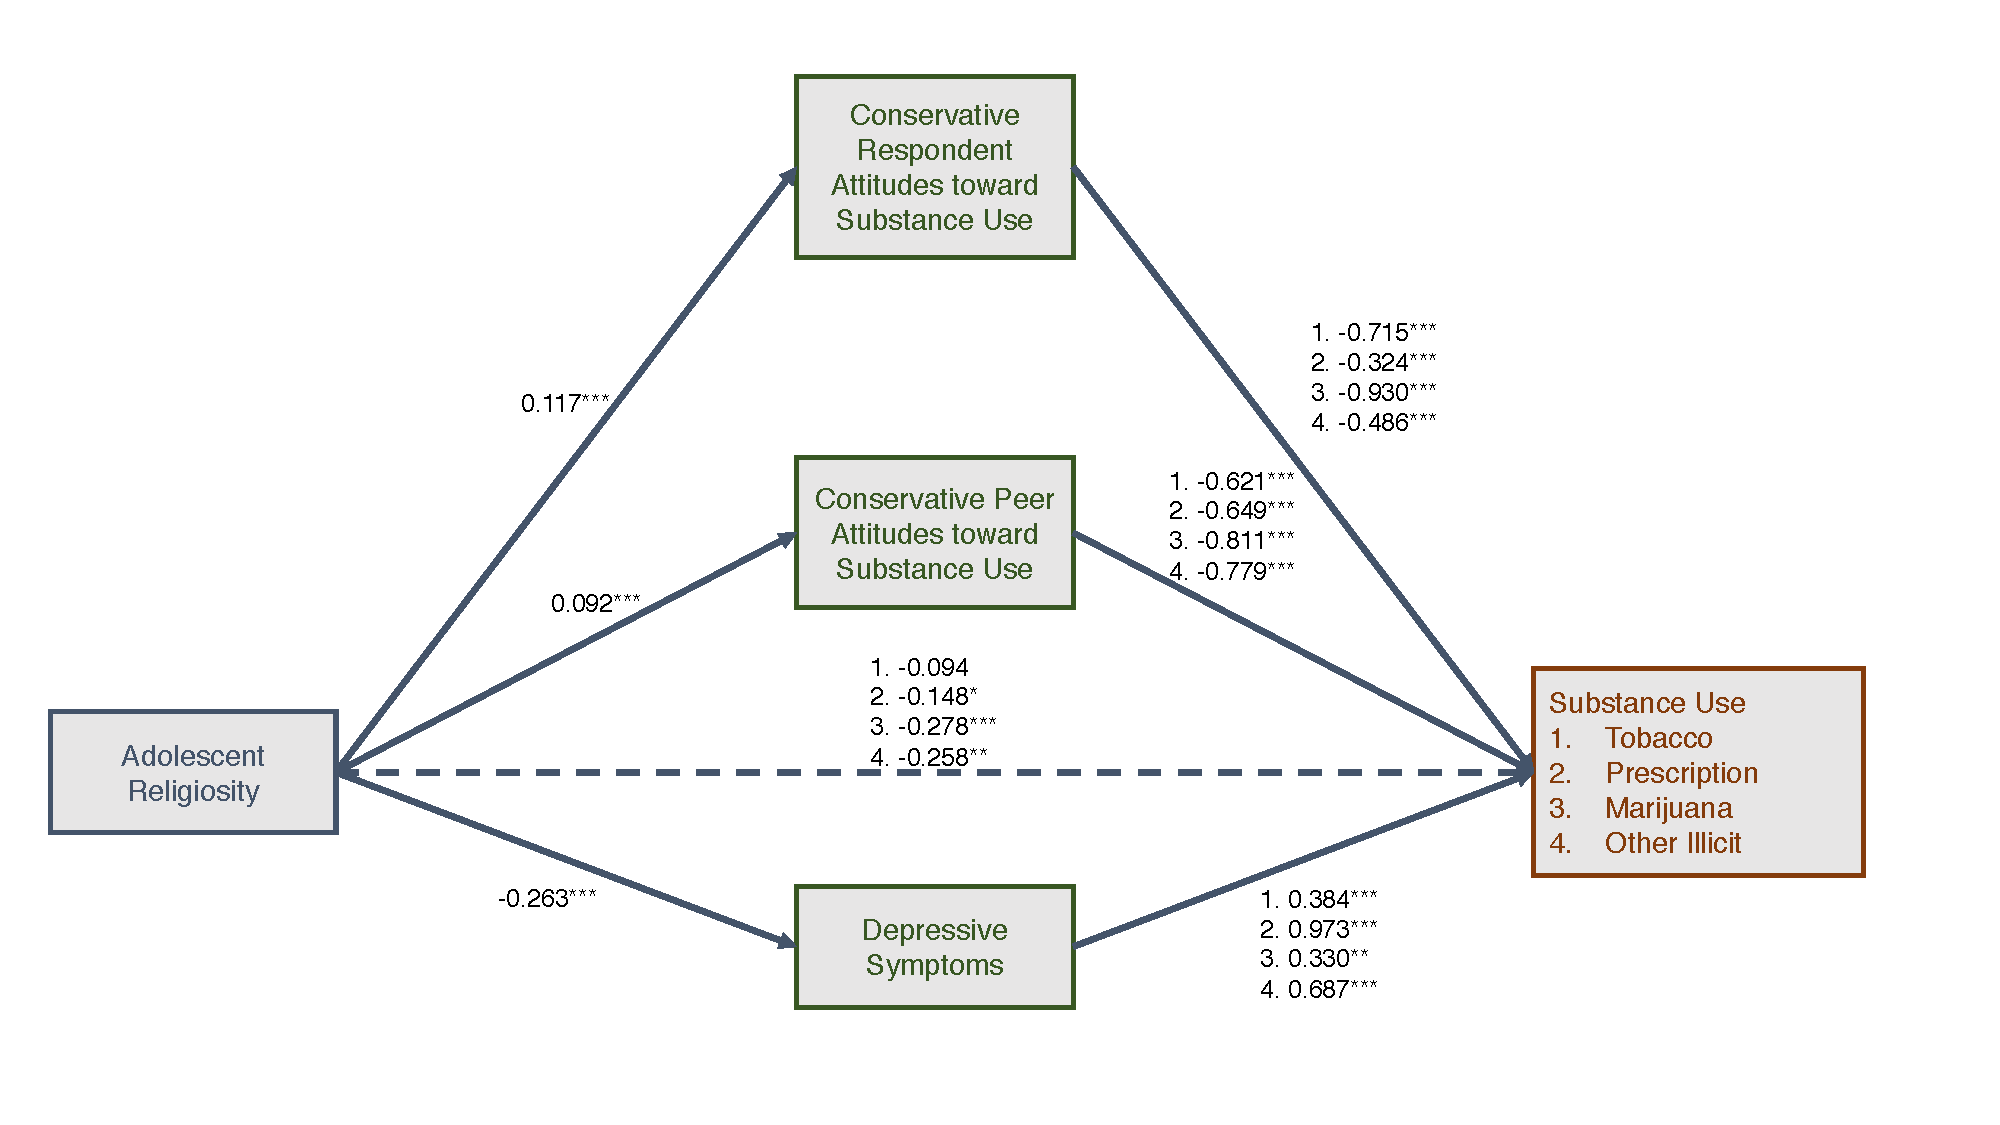
\includegraphics[width = \linewidth]{figures/fig_application_results.pdf}
\caption{Results of the mediation models' individual paths regarding religiosity and substance use. Note: *** p < .001, ** p < .01, * p < .05}
\label{fig:appresults}
\end{figure}

Because MMA provides information about each of the indirect effects
naturally in the same units, it is possible to assess the amount
mediated by each mediator while also controlling for the other mediators
in a straightforward manner---without having to fit several other models
and assess each \(c - c'\). Table \ref{tab:perc} presents the amount of
the total effect of religiosity on substance use that is mediated
through respondent conservative attitudes, peer conservative attitudes,
and depression. Overall, the effect of religiosity on substance use is
heavily mediated by the hypothesized mediators, more so for tobacco use
than the
others.\footnote{Using the approach used in Ford and Hill, the total mediated effects are slightly different than those estimated via the indirect and direct effects. This may be due to the weighting of the sample; an important area for further research into MMAs performance.}

\begin{table}[htb]
\centering
\caption{The percent of mediation (the percent of the total effect) by path for each outcome.}
\begin{tabular}{lcccc}
\toprule
            & \multicolumn{4}{c}{Outcome} \\
   Mediator & Tobacco & Prescription & Marijuana & Illicit \\ 
\midrule
Respondent Views  & 34.2  & 14.0  & 23.2 & 14.1 \\ 
Peer Views        & 23.2  & 22.0  & 15.8 & 17.7 \\ 
Depression        & 4.0   & 9.2   & 1.8  & 4.4 \\ 
Total Mediation   & 61.4  & 45.2  & 40.8 & 36.1 \\ 
\bottomrule
\end{tabular}\label{tab:perc}
\end{table}

In addition to this information, MMA provides information regarding the
indirect and direct effects in the same units. Figure \ref{fig:app}
highlights the indirect and direct effects with their associated 95\%
confidence intervals in the average marginal effects. All of the effects
here are in risk (probability) units---i.e., risk of tobacco use,
prescription misuse, marijuana use, or illicit drug use. Although all
indirect effects and most direct effects are significant, the effect
size estimates are particularly important here as the meaningfulness of
these significant effects can be overlooked.

These resulting effects are all small, with most effects less than 0.01
(i.e., less than a single risk unit). That is, most effects show changes
in the risk of the outcome by less than a single unit. For example, if
adolescent religiosity is increased by one unit, its effect on the risk
of tobacco use, through respondent attitudes, is a decrease of 0.007;
through peer attitudes a decrease of 0.005; through depression a
decrease of 0.001; and directly a decrease of 0.008. The total effect,
then, is approximately -0.021. Therefore, if an individual has a risk of
using tobacco at 50\%, by increasing religiosity by one unit (holding
the covariates constant), on average that individual's risk would
decrease to 47.9\%. About 0.013 of the effect of religiosity on tobacco
use is mediated while 0.008 is direct from religiosity. Ultimately,
these findings highlight the fact that the effect sizes, especially the
indirect and direct effect sizes, are valuable companions to the
p-values.

\begin{Shaded}
\begin{Highlighting}[]
\NormalTok{rbind_auto =}\StringTok{ }\ControlFlowTok{function}\NormalTok{(obj)\{}
  \KeywordTok{rbind}\NormalTok{(obj}\OperatorTok{$}\NormalTok{ind_effects[, }\DecValTok{3}\OperatorTok{:}\DecValTok{5}\NormalTok{] }\OperatorTok
\StringTok{          }\KeywordTok{set_names}\NormalTok{(}\KeywordTok{c}\NormalTok{(}\StringTok{"Estimate"}\NormalTok{, }\StringTok{"Lower"}\NormalTok{, }\StringTok{"Upper"}\NormalTok{)), }
\NormalTok{        fit_tob2}\OperatorTok{$}\NormalTok{dir_effects }\OperatorTok
\StringTok{          }\KeywordTok{set_names}\NormalTok{(}\KeywordTok{c}\NormalTok{(}\StringTok{"Estimate"}\NormalTok{, }\StringTok{"Lower"}\NormalTok{, }\StringTok{"Upper"}\NormalTok{)))}
\NormalTok{\}}
\KeywordTok{rbind}\NormalTok{(}\KeywordTok{rbind_auto}\NormalTok{(fit_tob2),}
      \KeywordTok{rbind_auto}\NormalTok{(fit_rx2),}
      \KeywordTok{rbind_auto}\NormalTok{(fit_mar2),}
      \KeywordTok{rbind_auto}\NormalTok{(fit_ill2)) }\OperatorTok
\StringTok{  }\NormalTok{xtable}\OperatorTok{::}\KeywordTok{xtable}\NormalTok{(}\DataTypeTok{digits =} \DecValTok{4}\NormalTok{) }\OperatorTok
\StringTok{  }\NormalTok{xtable}\OperatorTok{::}\KeywordTok{print.xtable}\NormalTok{()}
\end{Highlighting}
\end{Shaded}

\begin{Shaded}
\begin{Highlighting}[]
\NormalTok{p =}\StringTok{ }\KeywordTok{position_dodge}\NormalTok{(}\DataTypeTok{width =}\NormalTok{ .}\DecValTok{2}\NormalTok{)}
\NormalTok{inds }\OperatorTok
\StringTok{  }\KeywordTok{filter}\NormalTok{(type }\OperatorTok{==}\StringTok{ "Adjusted"}\NormalTok{) }\OperatorTok
\StringTok{  }\KeywordTok{ggplot}\NormalTok{(}\KeywordTok{aes}\NormalTok{(Path, Estimate, }\DataTypeTok{group =}\NormalTok{ type, }\DataTypeTok{color =}\NormalTok{ type)) }\OperatorTok{+}
\StringTok{    }\KeywordTok{geom_hline}\NormalTok{(}\DataTypeTok{yintercept =} \DecValTok{0}\NormalTok{, }\DataTypeTok{color =} \StringTok{"darkgrey"}\NormalTok{) }\OperatorTok{+}
\StringTok{    }\KeywordTok{geom_point}\NormalTok{(}\DataTypeTok{position =}\NormalTok{ p, }\DataTypeTok{alpha =}\NormalTok{ .}\DecValTok{8}\NormalTok{) }\OperatorTok{+}
\StringTok{    }\KeywordTok{geom_errorbar}\NormalTok{(}\KeywordTok{aes}\NormalTok{(}\DataTypeTok{ymin =}\NormalTok{ Lower, }\DataTypeTok{ymax =}\NormalTok{ Upper),}
                  \DataTypeTok{position =}\NormalTok{ p, }\DataTypeTok{alpha =}\NormalTok{ .}\DecValTok{8}\NormalTok{,}
                  \DataTypeTok{width =}\NormalTok{ .}\DecValTok{3}\NormalTok{) }\OperatorTok{+}
\StringTok{    }\KeywordTok{facet_wrap}\NormalTok{(}\OperatorTok{~}\NormalTok{Outcome) }\OperatorTok{+}
\StringTok{    }\KeywordTok{coord_flip}\NormalTok{() }\OperatorTok{+}
\StringTok{    }\NormalTok{anteo}\OperatorTok{::}\KeywordTok{theme_anteo_wh}\NormalTok{() }\OperatorTok{+}
\StringTok{    }\KeywordTok{theme}\NormalTok{(}\DataTypeTok{legend.position =} \StringTok{"bottom"}\NormalTok{,}
          \DataTypeTok{axis.line =} \KeywordTok{element_line}\NormalTok{(}\DataTypeTok{color =} \StringTok{"darkgrey"}\NormalTok{),}
          \DataTypeTok{panel.spacing =} \KeywordTok{unit}\NormalTok{(.}\DecValTok{3}\NormalTok{, }\StringTok{"in"}\NormalTok{)) }\OperatorTok{+}
\StringTok{    }\KeywordTok{scale_color_manual}\NormalTok{(}\DataTypeTok{values =} \KeywordTok{c}\NormalTok{(}\StringTok{"chartreuse4"}\NormalTok{, }\StringTok{"coral2"}\NormalTok{),}
                       \DataTypeTok{guide =} \OtherTok{FALSE}\NormalTok{) }\OperatorTok{+}
\StringTok{    }\KeywordTok{labs}\NormalTok{(}\DataTypeTok{x =} \StringTok{""}\NormalTok{, }\DataTypeTok{y =} \StringTok{""}\NormalTok{,}
         \DataTypeTok{color =} \StringTok{""}\NormalTok{)}
\end{Highlighting}
\end{Shaded}

\begin{verbatim}
## Error in loadNamespace(name): there is no package called 'anteo'
\end{verbatim}

\section{Conclusions}\label{conclusions}

The replication highlighted several important facets of the important
work by Ford and Hill (2012). First, it simplifies the interpretation of
the model by using average marginal effects. Second, it highlighted the
effect sizes in terms of risk of substance use. This allowed the
relatively small effects to be understood, not only in their
significance, but in their meaning. Ultimately, MMA provided a more
straightforward approach and substantially more information for each
model than other mediation approaches.

\singlespacing


\end{document}
